%Notes on Object Detection available at : https://www.mdpi.com/2072-4292/12/1/143 

This article by Qian et al. aims to solve two issues prevalent in anchor-based detection methods:
first the loss of low level information when using only the highest level feature maps for the feature extraction of region proposal.
Secondly, existing metrics, such as \gls{iou}, are not able to measure the distance between two non overlapping bounding boxes. During training, the bounding box loss is not able to directly optimize this metric. 

The authors implements a new metric, the \gls{giou}, which is able to measure the distance between non-overlapping bounding boxes, along with a bounding box loss system that is able to directly optimize the new metric. A new \gls{mlff} is proposed, and incorporated into an existing network.

This allows the authors to reach state of the art performance on the NWPU VHR-10 dataset\cite{nwpu}.

\subsection{Architecture}
\subsubsection{General Network Architecture}
The network can use an arbitrary size image as an input. This image is fed into a \gls{fpn}, which acts as the backbone of the network. This \gls{fpn} outputs multi-scale feature maps at different levels. Those multi-scale feature maps are used by the \gls{mlff}, which pools features using RoIAlign\cite{resNet} across multiple levels and concatenates them along the channel dimension. The fused features are utilized for bounding box regression and classification. A novel \gls{giou} loss is proposed, instead of the smooth L1 loss.


\begin{figure}[h!]
  \centering
  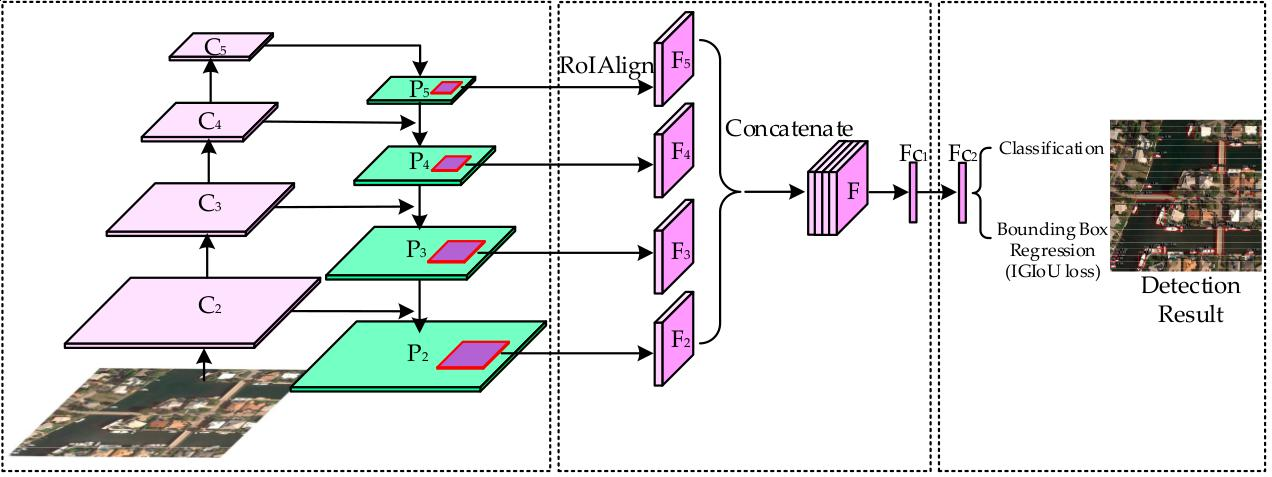
\includegraphics[width=\textwidth]{ODRSIArchi.jpg}
	\caption[General Architecture of the ODRSI]{Architecture of the proposed framework. The left part shows the feature pyramid network. Multilevel features fusion is shown in the middle, and classification and bounding box regression based on the IGIoU loss is shown in the rightmost part.}
  \label{fig:archiQian}
\end{figure}

\subsubsection{MLFF}
A novel \gls{mlff} module is proposed. The feature maps of all levels are used by a \gls{mlff} module for feature extraction. Each proposal generated by the \gls{fpn} are mapped to the feature maps of all levels. The size and location of the proposed region in the feature maps can be calculated based on the size ration between the proposal and the feature maps. 

Four regions of each proposal are transformed into four groups of $7 \times 7$ feature maps, denoted $F_2, F_3, F_4$ and $F_5$ in figure~\ref{fig:archiQian} using RoiAlign\cite{resNet}. The features are then concatenated along the channel dimension into a fused feature map called $F$.

Finally, a convolutional layer with a $7 \times 7$ kernel is used on $F$ to obtain $F_{C1}$ which is then passed to a fully connected layer.

\subsection{Generalized Intersection over Union}


A novel metric, the Generalized IoU (GIoU) is proposed to enhance the evaluation of proximity between two bounding boxes. The traditional \gls{iou} is insensitive to the scales of bounding boxes, and can be calculated using formula~\ref{eq:IoU}. Let $B_{GT}$ be the ground truth bounding box and $B_{PT}$ be the predicted bounding box.

\begin{equation}\label{eq:IoU}
	IoU = \frac{area(B_{GT} \cap B_{PT})}{area(B_{GT} \cup B_{PT})}
\end{equation}

The \gls{iou} is essentially the fraction of the intersection of the area of the predicted bounding box and the ground truth over the union of both bounding box. The \gls{iou} is not capable of measuring the distance when two bounding boxes are not overlapping. The introduced metric, address this issue.

The formula for the \gls{iou} is as follows:

\begin{equation}
	%Eq (5) in the original paper may have a typo where \cup is represented as U.......
	GIoU = IoU + \frac{area(B_{GT} \cup B_{PT})}{area(B_{EC})} - 1
\end{equation}

Where $B_{EC}$ represents the smallest enclosing box of $B_{GT}$ and $B_{PT}$. The \gls{iou} is inversely proportional to he distance between $B_{GT}$ and $B_{PT}$ where they are overlapping, but stays at 0 when they were not overlapping. The \gls{giou} is proportional to the distance of the two bounding boxes, and decreases with the distance between $B_{GT}$ and $B_{PT}$, whether or not the bounding boxes were overlapping.

\subsection{Bounding Box Regression based on Improved GIoU Loss (IGIoU)}
The bounding box regression loss used in traditional object detection methods is usually adopted to smooth the L1 or L2 loss. However, those two loss functions do not directly optimize the \gls{iou} metric. The smooth L1 or L2 loss are used to optimize the four parameters of the predicted bounding box, and the \gls{iou} is used to give more importance to the overlapping degree between the two bounding boxes. 

Integrating the value of the \gls{giou} into the loss can be done using formula~\ref{eq:giouloss} from Rezatofighi et al. \cite{giou}.

\begin{equation}
	\label{eq:giouloss}
		L_{GIoU} = 1 - GIoU
\end{equation}

This loss has a constant gradient during the training process, which restricts the effect of bounding box regression. The authors note that strength of the training should be enhanced when the predicted bounding box is far away from the ground truth, \textit{i.e.} the absolute value of the gradient should be higher when the \gls{giou} is small. Moreover, the value of the bounding box regression loss should decrease with the \gls{giou}. 

The improved GIoU Loss (IGIoU) is used to address those issues, and is given in the following formula:

\begin{equation}
	L_{IGIoU} = 2 \times log_2 - 2 \times log(1 + GIoU)
\end{equation}

\subsection{Results}
To validate the IGIoU loss and the \gls{mlff} module, quantitative comparisons were made between the proposed methods and five others methods on the NWPU VHR-10 dataset\cite{nwpu}. Those results are listed in table~\ref{tab:ODRSIcomparison}

The proposed method is also evaluated against four state of the art methods on the NWPU VHR-10 datasets, and are listed in table~\ref{tab:ODRSIcomparison}. 

\begin{table}[h!]
	\centering
	\begin{tabular}{@{}lllllll@{}}
		\toprule
		Method       &               & GIoU          &               &               & IoU           &               \\ \cmidrule(l){2-7} 
		             & mAP (\%)      & AP50(\%)      & AP75(\%)      & mAP(\%)       & AP50(\%)      & AP75(\%)      \\ \midrule
			     Faster R-CNN & 53.5          & 86.8          & 61.0          & 54.6          & 87.1          & 62.6          \\
			     Mask R-CNN   & 54.7          & 88.8          & 62.6          & 55.8          & 89.4          & 64.2          \\
			     \gls{fpn}          & 55.3          & 88.8          & 64.0          & 56.5          & 89.3          & 65.9          \\
			     PANet        & 56.3          & \textbf{90.5} & 63.9          & 57.8          & \textbf{91.8} & 65.8          \\
			     Proposed Method& \textbf{58.0} & \textbf{90.5} & \textbf{67.5} & \textbf{59.2} & 91.4          & \textbf{69.6} \\ \bottomrule
	\end{tabular}
	\caption{Comparison of the ODRSI against four existing detection framework on the NWPU VHR-10}
	\label{tab:ODRSIcomparison}
\end{table}

The method obtains state of the art results and better precision scores than all of the other tested methods, except in one case. 

\clearpage
